\documentclass[tikz,border=8pt,multi=tikzpicture]{standalone}
\usepackage{amsmath}
\usepackage{xcolor}
\usetikzlibrary{arrows.meta, calc}

\definecolor{mainblue}{HTML}{001158}
\definecolor{accent}{HTML}{8592bc}
\definecolor{lightaccent}{HTML}{e7e9f2}

\tikzset{
  force/.style={-{Stealth[length=3mm]}, line width=1.2pt, color=mainblue},
  dim/.style={-{Stealth[length=2mm]}, line width=0.7pt, color=accent},
  moment/.style={-{Stealth[length=2.5mm]}, line width=1.2pt, color=mainblue},
  qload/.style={-{Stealth[length=2mm]}, line width=0.9pt, color=mainblue!70},
  every node/.append style={font=\sffamily}
}

\newcommand{\festlager}[1]{
  \begin{scope}[shift={#1}]
    \draw[line width=1pt] (0,0) -- (-0.3,-0.5) -- (0.3,-0.5) -- cycle;
    \draw[line width=1pt] (-0.42,-0.5) -- (0.42,-0.5);
    \foreach \x in {-0.42,-0.24,...,0.42} {\draw[line width=0.4pt] (\x,-0.5) -- (\x-0.13,-0.68);}
  \end{scope}
}
\newcommand{\loslager}[1]{
  \begin{scope}[shift={#1}]
    \draw[line width=1pt] (0,0) -- (-0.3,-0.5) -- (0.3,-0.5) -- cycle;
    \foreach \x in {-0.18,0,0.18} {\draw[fill=white, line width=0.7pt] (\x,-0.6) circle (0.1);}
    \draw[line width=1pt] (-0.42,-0.72) -- (0.42,-0.72);
    \foreach \x in {-0.42,-0.24,...,0.42} {\draw[line width=0.4pt] (\x,-0.72) -- (\x-0.13,-0.9);}
  \end{scope}
}
\newcommand{\einspannung}[1]{
  \begin{scope}[shift={#1}]
    \draw[mainblue, line width=1.5pt] (0,0.6) -- (0,-0.6);
    \foreach \y in {-0.5,-0.25,...,0.5} {\draw[line width=0.5pt] (0,\y) -- (-0.25,\y+0.22);}
  \end{scope}
}
\newcommand{\gelenk}[1]{
  \begin{scope}[shift={#1}]
    \draw[draw=mainblue, fill=white, line width=1.3pt] (0,0) circle (0.13);
  \end{scope}
}
\newcommand{\qarrows}[4]{
  \draw[mainblue!70, line width=0.8pt] (#1,#3) -- (#2,#3);
  \pgfmathsetmacro{\qn}{int(round((#2-#1)/0.5))}
  \foreach \i in {0,...,\qn} {
    \pgfmathsetmacro{\qx}{(#1)+\i*0.5}
    \draw[qload] (\qx,#3) -- (\qx,#3-#4);
  }
}

\begin{document}

% ================= Concept: hinge transmits force, not moment =================
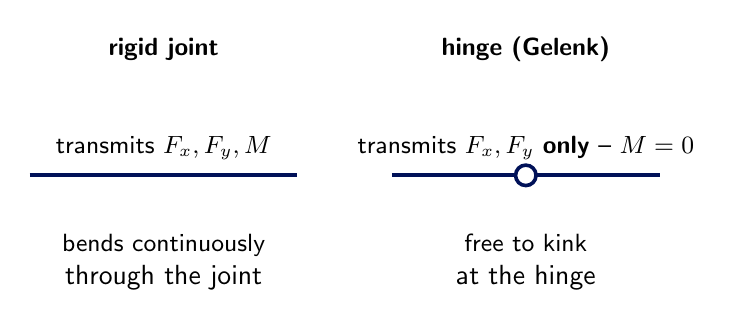
\begin{tikzpicture}
\node[align=center] at (-1.3,1.6) {\small \textbf{rigid joint}};
\draw[mainblue, line width=1.5pt] (-3,0) -- (0.4,0);
\node at (-1.3,0.35) {\small transmits $F_x,F_y,M$};
\node[align=center] at (3.3,1.6) {\small \textbf{hinge (Gelenk)}};
\draw[mainblue, line width=1.5pt] (1.6,0) -- (5,0);
\gelenk{(3.3,0)}
\node at (3.3,0.35) {\small transmits $F_x,F_y$ \textbf{only} -- $M=0$};
\node[align=center] at (-1.3,-1.1) {\small bends continuously\\ through the joint};
\node[align=center] at (3.3,-1.1) {\small free to kink\\ at the hinge};
\end{tikzpicture}

% ================= Concept: cutting at the hinge =================
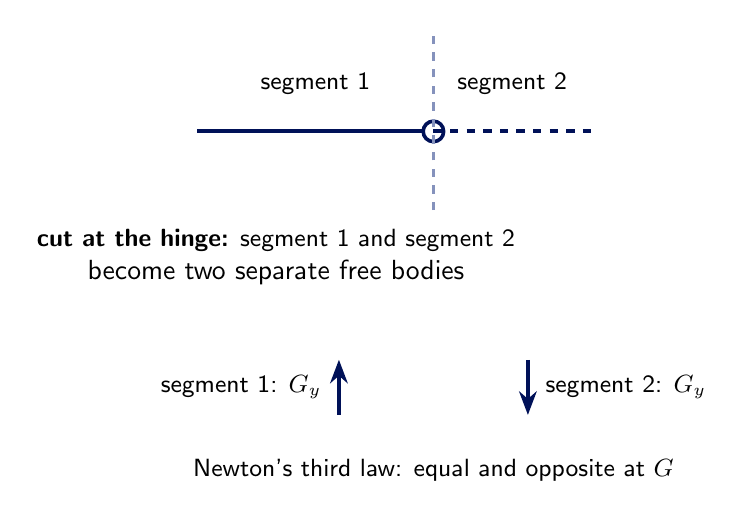
\begin{tikzpicture}
\draw[mainblue, line width=1.5pt] (0,0) -- (3,0);
\gelenk{(3,0)}
\draw[mainblue, line width=1.5pt, dashed] (3,0) -- (5,0);
\node[align=center] at (1.5,0.6) {\small segment 1};
\node[align=center] at (4,0.6) {\small segment 2};
\draw[accent, dashed, line width=1pt] (3,-1.0) -- (3,1.3);
\node[align=center] at (1.0,-1.6) {\small \textbf{cut at the hinge:} segment 1 and segment 2\\ become two separate free bodies};
\draw[force] (1.8,-3.6) -- (1.8,-2.9);
\node[left] at (1.7,-3.25) {\small segment 1: $G_y$};
\draw[force] (4.2,-2.9) -- (4.2,-3.6);
\node[right] at (4.3,-3.25) {\small segment 2: $G_y$};
\node[align=center] at (3,-4.3) {\small Newton's third law: equal and opposite at $G$};
\end{tikzpicture}

% ================= Ex 7.1 problem: fixed + hinge + roller + overhang load =================
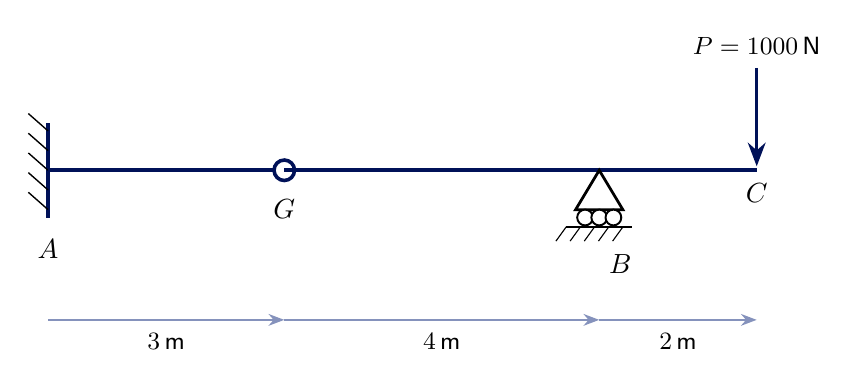
\begin{tikzpicture}
\einspannung{(0,0)}
\draw[mainblue, line width=1.5pt] (0,0) -- (3,0);
\gelenk{(3,0)}
\draw[mainblue, line width=1.5pt] (3,0) -- (9,0);
\loslager{(7,0)}
\node[below] at (0,-0.75) {$A$};
\node[below] at (3,-0.25) {$G$};
\node[below right] at (7,-0.95) {$B$};
\node[below] at (9,-0.05) {$C$};
\draw[force] (9,1.3) -- (9,0.05);
\node[above] at (9,1.35) {\small $P=1000\,\text{N}$};
\draw[dim] (0,-1.9) -- (3,-1.9);
\node[below] at (1.5,-1.95) {\small $3\,\text{m}$};
\draw[dim] (3,-1.9) -- (7,-1.9);
\node[below] at (5,-1.95) {\small $4\,\text{m}$};
\draw[dim] (7,-1.9) -- (9,-1.9);
\node[below] at (8,-1.95) {\small $2\,\text{m}$};
\end{tikzpicture}

% ================= Ex 7.1 split free bodies =================
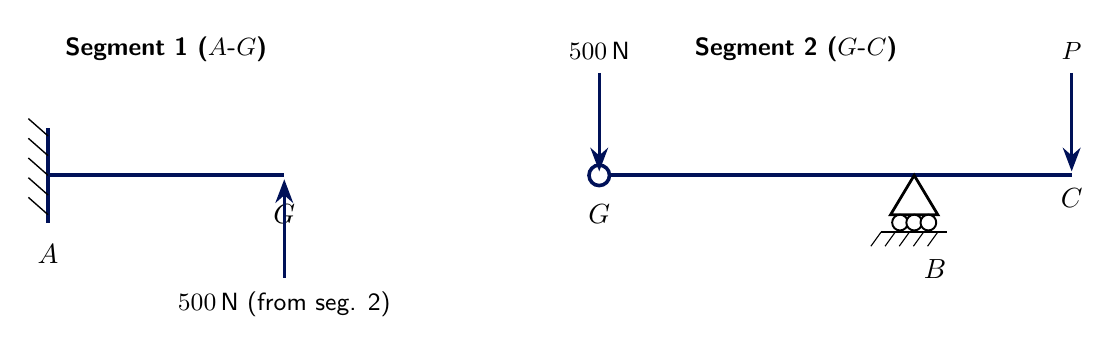
\begin{tikzpicture}
\node[align=center] at (1.5,1.6) {\small \textbf{Segment 1 ($A$-$G$)}};
\einspannung{(0,0)}
\draw[mainblue, line width=1.5pt] (0,0) -- (3,0);
\node[below] at (0,-0.75) {$A$};
\node[below] at (3,-0.25) {$G$};
\draw[force] (3,-1.3) -- (3,-0.05);
\node[below] at (3,-1.35) {\small $500\,\text{N}$ (from seg. 2)};
%
\node[align=center] at (9.5,1.6) {\small \textbf{Segment 2 ($G$-$C$)}};
\draw[mainblue, line width=1.5pt] (7,0) -- (13,0);
\gelenk{(7,0)}
\loslager{(11,0)}
\node[below] at (7,-0.25) {$G$};
\node[below right] at (11,-0.95) {$B$};
\node[below] at (13,-0.05) {$C$};
\draw[force] (7,1.3) -- (7,0.05);
\node[above] at (7,1.35) {\small $500\,\text{N}$};
\draw[force] (13,1.3) -- (13,0.05);
\node[above] at (13,1.35) {\small $P$};
\end{tikzpicture}

% ================= Ex 7.2 problem: pin + roller + hinge + roller, midspan load =================
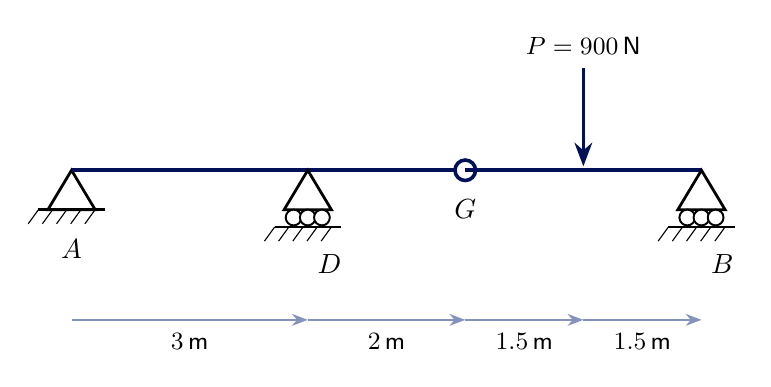
\begin{tikzpicture}
\festlager{(0,0)}
\draw[mainblue, line width=1.5pt] (0,0) -- (5,0);
\loslager{(3,0)}
\gelenk{(5,0)}
\draw[mainblue, line width=1.5pt] (5,0) -- (8,0);
\loslager{(8,0)}
\node[below] at (0,-0.75) {$A$};
\node[below right] at (3,-0.95) {$D$};
\node[below] at (5,-0.25) {$G$};
\node[below right] at (8,-0.95) {$B$};
\draw[force] (6.5,1.3) -- (6.5,0.05);
\node[above] at (6.5,1.35) {\small $P=900\,\text{N}$};
\draw[dim] (0,-1.9) -- (3,-1.9);
\node[below] at (1.5,-1.95) {\small $3\,\text{m}$};
\draw[dim] (3,-1.9) -- (5,-1.9);
\node[below] at (4,-1.95) {\small $2\,\text{m}$};
\draw[dim] (5,-1.9) -- (6.5,-1.9);
\node[below] at (5.75,-1.95) {\small $1.5\,\text{m}$};
\draw[dim] (6.5,-1.9) -- (8,-1.9);
\node[below] at (7.25,-1.95) {\small $1.5\,\text{m}$};
\end{tikzpicture}

% ================= Ex 7.2 split free bodies =================
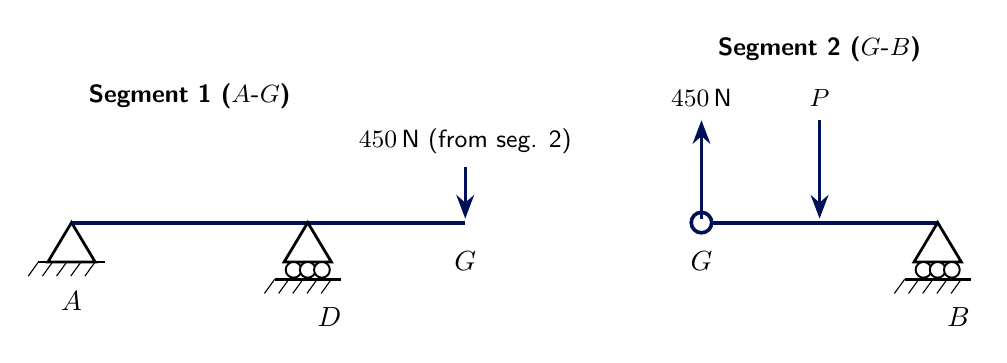
\begin{tikzpicture}
\node[align=center] at (1.5,1.6) {\small \textbf{Segment 1 ($A$-$G$)}};
\festlager{(0,0)}
\draw[mainblue, line width=1.5pt] (0,0) -- (5,0);
\loslager{(3,0)}
\node[below] at (0,-0.75) {$A$};
\node[below right] at (3,-0.95) {$D$};
\node[below] at (5,-0.25) {$G$};
\draw[force] (5,0.7) -- (5,0.05);
\node[above] at (5,0.75) {\small $450\,\text{N}$ (from seg. 2)};
%
\node[align=center] at (9.5,2.2) {\small \textbf{Segment 2 ($G$-$B$)}};
\draw[mainblue, line width=1.5pt] (8,0) -- (11,0);
\gelenk{(8,0)}
\loslager{(11,0)}
\node[below] at (8,-0.25) {$G$};
\node[below right] at (11,-0.95) {$B$};
\draw[force] (8,0.05) -- (8,1.3);
\node[above] at (8,1.35) {\small $450\,\text{N}$};
\draw[force] (9.5,1.3) -- (9.5,0.05);
\node[above] at (9.5,1.35) {\small $P$};
\end{tikzpicture}

% ================= Ex 7.3 problem: fixed + hinge + UDL over whole span 2 + roller + overhang =================
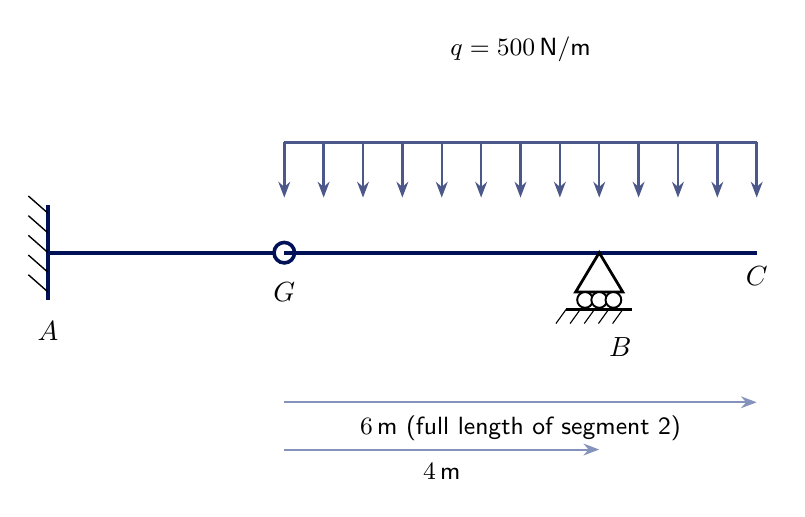
\begin{tikzpicture}
\einspannung{(0,0)}
\draw[mainblue, line width=1.5pt] (0,0) -- (3,0);
\gelenk{(3,0)}
\draw[mainblue, line width=1.5pt] (3,0) -- (9,0);
\loslager{(7,0)}
\node[below] at (0,-0.75) {$A$};
\node[below] at (3,-0.25) {$G$};
\node[below right] at (7,-0.95) {$B$};
\node[below] at (9,-0.05) {$C$};
\qarrows{3}{9}{1.4}{0.7}
\node[above] at (6,2.3) {\small $q=500\,\text{N/m}$};
\draw[dim] (3,-1.9) -- (9,-1.9);
\node[below] at (6,-1.95) {\small $6\,\text{m}$ (full length of segment 2)};
\draw[dim] (3,-2.5) -- (7,-2.5);
\node[below] at (5,-2.55) {\small $4\,\text{m}$};
\end{tikzpicture}

% ================= Ex 7.3 split free bodies =================
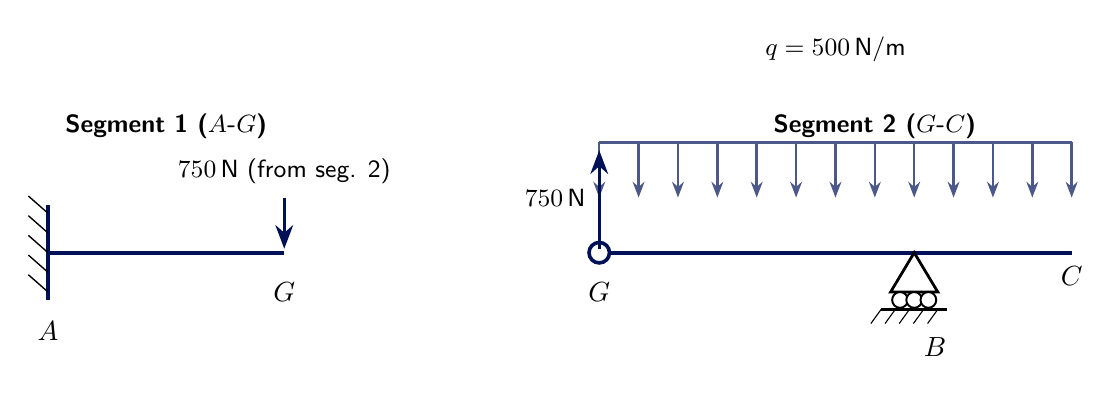
\begin{tikzpicture}
\node[align=center] at (1.5,1.6) {\small \textbf{Segment 1 ($A$-$G$)}};
\einspannung{(0,0)}
\draw[mainblue, line width=1.5pt] (0,0) -- (3,0);
\node[below] at (0,-0.75) {$A$};
\node[below] at (3,-0.25) {$G$};
\draw[force] (3,0.7) -- (3,0.05);
\node[above] at (3,0.75) {\small $750\,\text{N}$ (from seg. 2)};
%
\node[align=center] at (10.5,1.6) {\small \textbf{Segment 2 ($G$-$C$)}};
\draw[mainblue, line width=1.5pt] (7,0) -- (13,0);
\gelenk{(7,0)}
\loslager{(11,0)}
\node[below] at (7,-0.25) {$G$};
\node[below right] at (11,-0.95) {$B$};
\node[below] at (13,-0.05) {$C$};
\qarrows{7}{13}{1.4}{0.7}
\node[above] at (10,2.3) {\small $q=500\,\text{N/m}$};
\draw[force] (7,0.05) -- (7,1.3);
\node[left] at (6.95,0.7) {\small $750\,\text{N}$};
\end{tikzpicture}

\end{document}
